\newif\ifrevtex
\revtextrue

\ifrevtex
    \documentclass[aps,prd,final,twocolumn,letterpaper,nofootinbib]{revtex4-1}
\else
    \documentclass[twocolumn]{article}
\fi

%\usepackage[letterpaper,hmargin=0.8in,vmargin=0.8in]{geometry}
\usepackage{graphicx}

\usepackage{amsmath,amssymb}
\usepackage{siunitx}


%\usepackage{mathpazo}
\usepackage{microtype}

\usepackage{diagbox}
\usepackage{multirow}

\usepackage{color}
%\usepackage[printwatermark]{xwatermark}
%\newwatermark[allpages,color=red!10,angle=45,scale=3,xpos=0,ypos=0]{DRAFT}

\usepackage{tikz}

\usepackage{hyperref}
\usepackage{cleveref}


\usepackage{etoolbox} % for \appto

\makeatletter
\appto{\appendix}{%
  \@ifstar{\def\thesection{\unskip}\def\theequation@prefix{A.}}%
          {\def\thesection{\Alph {section}}}%
}
\makeatother


\newcommand\RR{\mathbb{R}}
\DeclareMathOperator\im{im}

\newcommand{\abs}[1]{|#1|}


\newcommand{\mb}{\mathbf}

%\usepackage{tikz}
%\usetikzlibrary{arrows}
%\usetikzlibrary{angles,patterns,calc}

\newcommand\headers{
    \title{Rigiditea: web-based rigidity algorithms}
    \author{Tony Zhang and Menghua Wu}
    \date{May 17, 2017}    
    \begin{abstract}
        We present Rigiditea,
        a native client-side web-based implementation of two algorithms
        for testing generic rigidity of graphs:
        the $n$-dimensional randomized infinitesimal-rigidity-based algorithm
        and the deterministic pebble game algorithm for two-dimensional rigidity.
        For the latter, we provide a step-by-step visualization of the algorithm
        for aid in understanding the algorithm.
    \end{abstract}
}


\ifrevtex\relax\else\headers\fi
\begin{document}
\ifrevtex\headers\fi

\maketitle



% % % % % % % % % %
%    INTRODUCTION
% % % % % % % % % %

\tableofcontents

\section{Introduction}

The theory of linkages has long been of interest
not only for its mathematical appeal
but also for its many obvious applications;
indeed, linkages have been used to model everything
from trusses to robot arms to proteins.
An obvious question that arises is that of \emph{rigidity}:
whether a linkage can move at all.

It's not hard to see that rigidity depends on more than
the combinatorial structure of the linkage
(usually specified as an undirected graph).
The number of dimensions in which we embed the linkage
and the particular configuration of the linkage
affects its rigidity.

Fortunately, if we only consider \emph{generic} embeddings
(which we take for simplicity to mean
there are no algebraic dependences between coordinates),
rigidity (and more generally, the number of degrees of freedom)
becomes a function only of the graph and the embedding dimension.

We implemented two major algorithms for determining generic rigidity,
as well as a web-based interface for interacting with them.
The first algorithm, which works for arbitrarily many dimensions~$d$,
considers a random embedding of the graph into $\RR^d$
and computes the number of \emph{infinitesimal} degrees of freedom (dof)
as described in \cite[\S4.4.2]{gfalop}.
The second is the famous \emph{pebble game algorithm},
first introduced by Jacobs and Hendrickson in 1997~\cite{jacobs97}.

To the best of our knowledge,
there did not exist convenient implementations of
either rigidity algorithm.
In particular,
we were unable to find any implementation of the infinitesimal algorithm,
and only found a Java applet for the pebble game \cite{stjohnapplet}.

Let us outline the remainder of this paper.
In \cref{sec:arch}, we describe the structure of our web application.
We next develop the theory behind the two rigidity algorithms
in \cref{sec:pebble,sec:infrigid}
to the level of detail necessary for understanding our work.
(Notably, we introduce a correction in \cref{sec:infrigid}
to the well-known formula for the infinitesimal dof of a linkage.)
We conclude with a comparison of to the existing Java applet
and a discussion of possible extensions to Rigiditea in \cref{sec:discuss}.

\section{Architecture}
\label{sec:arch}

We provide a high-level overview of our web application
and algorithms to acquaint users with Rigiditea.
All of our code was written in CoffeeScript,
which was transpiled down to JavaScript.
Thus, our entire app runs in the browser.
Still, there was a clear divide between user interface code
and ``backend," algorithmic code.

\subsection{Interface}

\begin{figure}[ht]
\begin{tikzpicture}
\node at (0,0) {
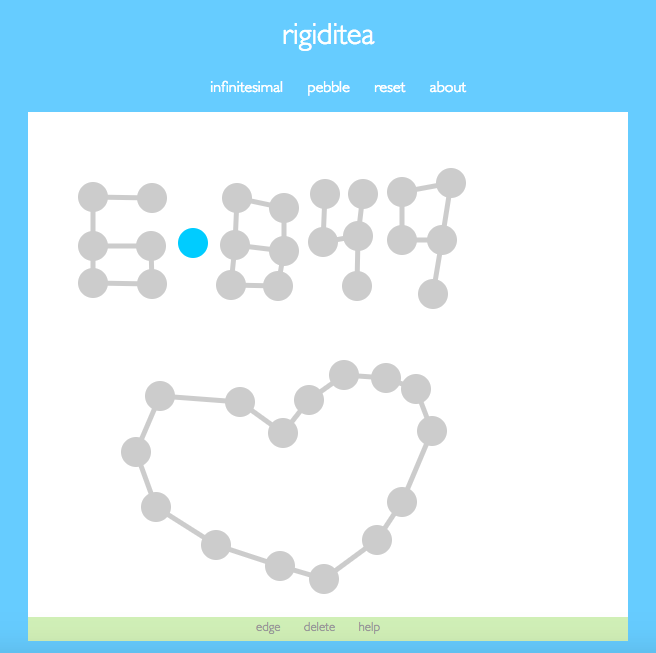
\includegraphics[scale=.3]{img/ui}
};
\draw (-3,-2.7) rectangle (3,2);
\node at (0,-1.5) {\large graph-drawing canvas};

\draw (-2,2.2) rectangle (2,2.7);
\node at (-2.5,2.45) {menu};

\draw (-1.5,-3) rectangle (1.5,-3.3);
\node at (-2.4,-3.15) {controls};
\end{tikzpicture}
\caption{High level overview of graphical user interface.
We aimed for a simple, but powerful design.}
\label{fig:ui}
\end{figure}

We built an intuitive and aesthetically-pleasing
graphical user interface (GUI)
to create and analyze linkages as 2D planar graphs.
We outline the main components of our GUI in \cref{fig:ui}.

Users may click anywhere on the canvas to add a new node to the graph.
After creating nodes,
users can interact with the interface
through either the menu bar or the control panel.
The former focuses on algorithm running and general information,
while the latter is tailored towards graph creation.
\Cref{fig:ui} identifies these elements in the actual interface.
In addition to the menu and control panel,
we also provide keyboard shortcuts to streamline the user experience.
\Cref{tab:menu} enumerates the various commands available,
their functionalities, and keyboard shortcuts.

\begin{table}[ht]
\caption{Control panel items and descriptions.}
\def\arraystretch{1.5}
\begin{tabular}{c | c | p{0.5\linewidth} | c}
& item & description & key \\ \hline
\multirow{3}{.5cm}{\rotatebox{90}{menu bar items~~}}
& pebble & advances pebble algorithm one step
(one cover enlargement; see \cref{sec:pebble}) & $\to$\\
& reset & resets defaults, initializes new graph, wipes canvas & r \\
& about & background information about algorithms,
web application, and further reading & a \\\hline
\multirow{3}{.5cm}{\rotatebox{90}{control panel~~}} &
edge & draws an edge between two selected vertices & e\\
& delete & deletes all selected components, including incident edges
to selected nodes & x \\
& help & provides information about graph designing interface,
including keyboard shortcuts & h \\
\end{tabular}
\label{tab:menu}
\end{table}

The GUI was created using the open-source library \texttt{d3.js},
one of the most widely used for data visualization.
Conveniently, \texttt{d3} allowed us to link graph data objects
directly to SVG elements on the canvas.

\subsection{Graph representation}

Graphs were represented as custom Javascript \texttt{Graph} objects,
each with a list of \texttt{Node} objects,
a list of \texttt{Edge} objects,
and other specialized instance methods,
such as the infinitesimal-rigidity-based generic rigidity algorithm.

Each \texttt{Edge} object keeps track of
its unique \texttt{id},
\texttt{source} and \texttt{target} \texttt{Node} objects,
and miscellaneous \texttt{attributes},
such as current and previous color.
The \texttt{Node} objects
each possess a unique \texttt{id}, \texttt{x} and \texttt{y} coordinates,
and a map of \texttt{attributes}.
All unique \texttt{id}s mentioned above are randomly generated,
case-sensitive alphanumeric strings of 5 characters.
We provide an example \texttt{Graph} in \Cref{fig:graphrep}.


We use an absolute pixel-based coordinate system to position nodes.
Each \texttt{Node} keeps track of its own location on the canvas.
\texttt{Edge} objects are then drawn to connect its endpoints.
All elements also keep track of their own colors,
which change upon selection
or visualization of the pebble algorithm,
as we shall discuss.

\begin{figure}[ht]
\begin{verbatim}
Graph: {
   nodes: {
     Node:
       {id: a6849, x:68, y:49, attr: {fill: #CEF}},
     Node:
       {id: b6867, x:68, y:67, attr: {fill: #FCE}}},
   edges: {
     Edge:
       {source: Node, target: Node,
         attr: {stroke: #CEF}}},
         ...
   [instance methods]
}
\end{verbatim}
\caption{Possible representation of the graph $K_2$ (two nodes joined with a single edge) as a \texttt{Graph}.}
\label{fig:graphrep}
\end{figure}

We also implemented a child \texttt{PebbleGraph} class,
whose additional data structures and instance methods
allow us to run (and in particular, to step through) the pebble algorithm.
%\texttt{PebbleGraph} objects can be easily created
%from standard \texttt{Graph} objects since
%their underlying representations are the same.
In particular, \texttt{PebbleGraph} objects also track
assignments of ``pebbles'' to edges and vertices
(as we shall explain).
Once we start the pebble game algorithm,
of course, we cannot continue mutating the combinatorial structure of the graph.
Thus, once we begin running the algorithm,
we disable graph editing in the GUI
and generate a \texttt{PebbleGraph}.

\section{Pebble game visualization}
\label{sec:pebble}

We shall sketch the pebble game algorithm
for generic two-dimensional rigidity testing
and describe our visualization for it.
For a more detailed exposition on the algorithm,
we refer the reader to the original paper~\cite{jacobs97}.

\subsection{The algorithm}

Before describing the algorithm,
we present some basic definitions.
Consider undirected graph $G = (V, E)$
with $n$ vertices and $m$ edges.
We say a subset of the edges is \emph{independent}
if they produce independent constraints on the motion of the vertices
in a generic embedding.
An independent set is \emph{maximal} if we can't add another edge
while preserving independence.

In two dimensions, $n$ unconstrained vertices have $2n-3$ degrees of freedom,
where we have excluded rigid motion.
Now each independent edge reduces this freedom by one,
so that
\[
    \text{dof} = 2n - 3 - \abs{\text{maximal independent set}}.
\]
It follows that our graph is generically rigid
if and only if we can find $2n-3$ independent edges.\footnote{It makes sense
to talk about \emph{the} size 
of maximal independent sets
for the same reason that the dimension of a span of vectors
is independent of the order in which we consider them;
indeed, edges correspond to vectors in $\RR^{dn}$,
as we shall see in the next section.}

On a high level,
the pebble algorithm builds an independent set of edges $\hat E$
by arbitrarily ordering the edges
and accepting an edge into $\hat E$
if and only if doing so would preserve independence.
Of course, we initialize $\hat E = \varnothing$.
After all edges are considered,
we have a maximal independent set,
so testing rigidity becomes a simple matter.

The key insight of the algorithm
is the observation that we can test independence of a new edge $e$
and the current independent set $\hat E$
by playing the namesake pebble game,
which we now describe, largely following \cite{stjohnapplet}.

Each vertex is given two pebbles it can use to cover incident edges.
At any given moment, we are attempting to add some edge $e$
to the partially-built independent set~$\hat E$.
We begin with a pebble covering such that all edges in $\hat E$
are covered by at least one pebble.

To test independence of $e$,
it actually suffices to check whether we can \emph{enlarge} the covering of $\hat E$
to a covering of $\hat E \cup \{e\}$
such that $e$ is covered by \emph{four} pebbles,
while keeping all of $\hat E$ covered.

To find such a covering,
we define the following enlargement subroutine,
which tries to find an extra pebble to cover $e = (u, v)$.
Starting at endpoint $u$,
we look for a vertex or an edge with a free pebble
(that is, a pebble not covering an edge
or one redundantly covering an edge)
via depth-first search.
Should we find a free pebble,
we rearrange pebbles along the path so that $e$ has an extra pebble.
Otherwise, we attempt the same operation on $v$.

If we cannot successfully apply this subroutine four times to $e$,
we discard $e$ from consideration.
Otherwise, we add it to $\hat E$ and consider a new $e$.
As a result,
we see that this algorithm runs in $O(mn)$ time.
We have $O(m)$ iterations,
each of which involves at most four $O(n)$ depth-first searches.
In practice, we did not bother with making our implementation particularly efficient,
since GUI rendering proved to be our performance bottleneck.


\subsection{Visualization}

\begin{figure}[h]
   \centering
   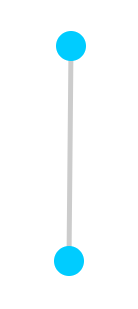
\includegraphics[width=.19\linewidth]{img/l1}
   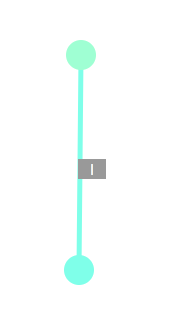
\includegraphics[width=.19\linewidth]{img/l2}
   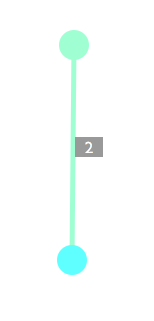
\includegraphics[width=.19\linewidth]{img/l3}
   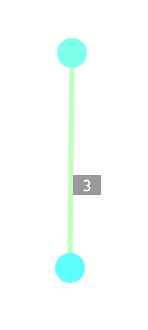
\includegraphics[width=.19\linewidth]{img/l4}
   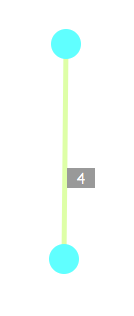
\includegraphics[width=.19\linewidth]{img/l5}
   \caption{Pebble cover on a single segment.
   We start by drawing the segment
   and proceed to cover it with pebbles,
   until determining that a segment is rigid.
   Note the color change on the endpoints
   as their pebbles are allocated to the edge.}
   \label{fig:seg}
\end{figure}

Rigiditea primarily provides a visualization of the pebble game algorithm.
In particular, it allows the user to trigger individual cover enlargement steps.
Edges and vertices are color-coded by the number of pebbles covering them,
making it clear which edges we've added to $\hat E$
(those always covered by pebbles)
and which edge $e$ we're adding
(the one accumulating pebbles).
We use a spectrum of blue and green,
where zero pebbles is a darker blue and four pebbles is a light yellow-green.
\Cref{fig:seg} shows a simplified version of this process for a single segment,
and \cref{fig:pebbles} demonstrates multiple phases of the algorithm
for a triangle.

For additional clarity,
a user can view the number of pebbles on an edge or node
at any given point during the pebble game
by mousing over that element.

\begin{figure*}[t]
   \centering
   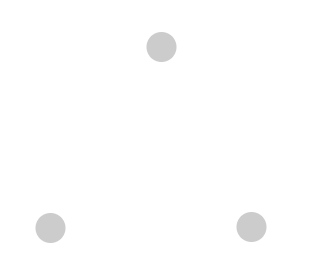
\includegraphics[width=.24\linewidth]{img/t1}
   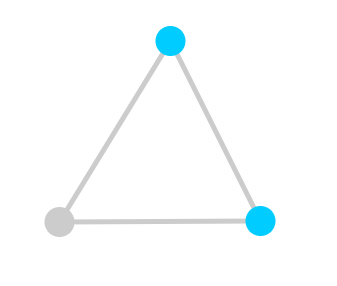
\includegraphics[width=.24\linewidth]{img/t2}
   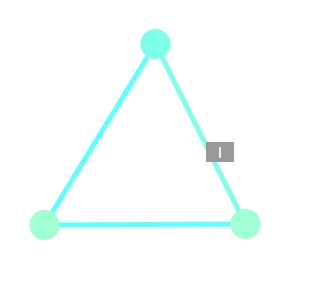
\includegraphics[width=.24\linewidth]{img/t3}
   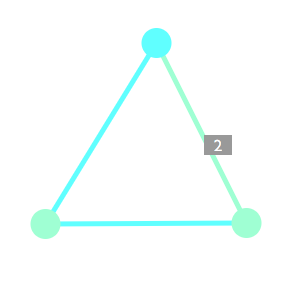
\includegraphics[width=.24\linewidth]{img/t4}
   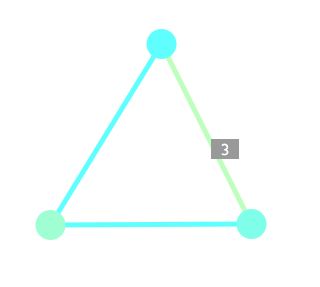
\includegraphics[width=.24\linewidth]{img/t5}
   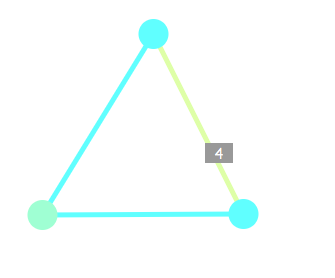
\includegraphics[width=.24\linewidth]{img/t6}
   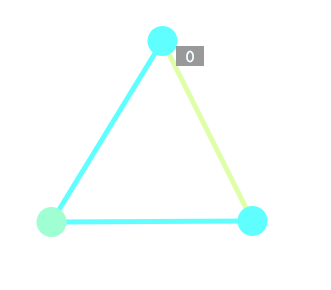
\includegraphics[width=.24\linewidth]{img/t7}
   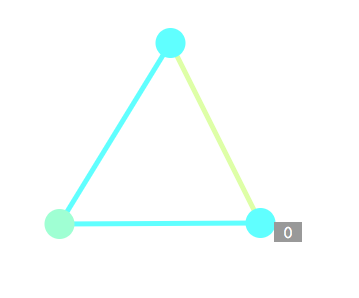
\includegraphics[width=.24\linewidth]{img/t8}
   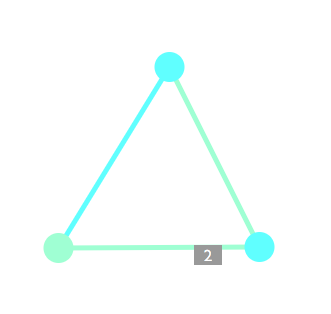
\includegraphics[width=.24\linewidth]{img/t9}
   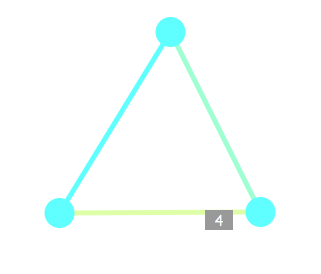
\includegraphics[width=.24\linewidth]{img/t10}
   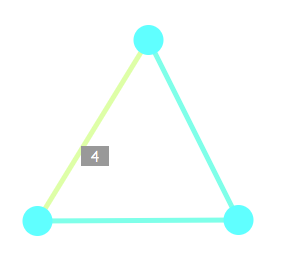
\includegraphics[width=.24\linewidth]{img/t11}
   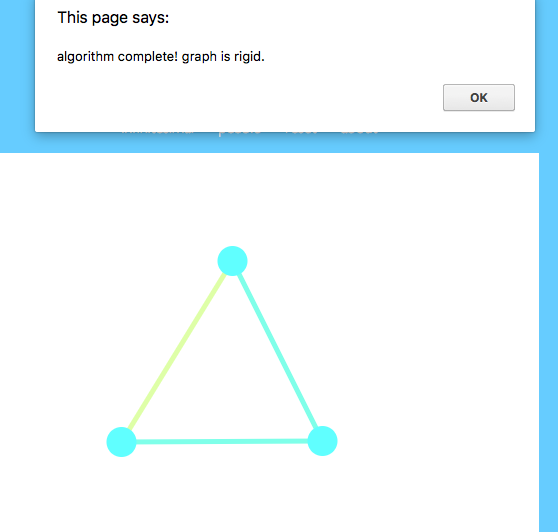
\includegraphics[width=.24\linewidth]{img/t12}
   \caption{Process of a single pebble game for a triangle.
   The labels on each edge or node show the number of pebbles on that element.
   We can see that the number of pebbles increases each time from 1 to 4,
   as the pebbles on nodes are transferred to edges.
   In the final frame, we see that the triangle is successfully identified as rigid.}
   \label{fig:pebbles}
\end{figure*}

\section{Infinitesimal rigidity}
\label{sec:infrigid}

In this section,
we outline the algorithm for determining the infinitesimal degrees of freedom
of a $d$-dimensional linkage embedding.
The algorithm is straightforwardly presented in \cite[\S4.4.2]{gfalop},
so we only provide a brief sketch.
More importantly, however,
we shall prove a correction to the formula the algorithm uses
to compute the infinitesimal degrees of freedom.

As before, suppose we have $G = (V, E)$ of $n$ vertices and $m$ edges.
Given a $d$-dimensional embedding of the vertices,
each edge provides a linear constraint
on the allowed infinitesimal motions of $V$.
In matrix form, we can write
\begin{equation}
    R\mb v = 0
\end{equation}
for a \emph{rigidity matrix}~$R$ of shape $dn \times m$
and an infinitesimal motion $\mb v \in \RR^{dn}$,
whose components are the $d$ components
of the infinitesimal motion of each of $n$ vertices.

The space of allowed infinitesimal motions is then $\ker R$.
However, some of these motions are rigid,
corresponding to the infinitesimal generators of rigid motions in $\RR^d$,
which form a $\binom{d+1}{2}$-dimensional vector space:
the Lie algebra $\mathfrak{se}(d)$ of the \emph{special Euclidean group},
the orientation-preserving isometry group of $\RR^d$.

Once we exclude these trivial motions,
we would naively expect the subspace of nontrivial infinitesimal motions
to have dimension
\begin{equation}\label{eq:wrong-infdof}
    \dim\ker R - \binom{d+1}{2} = dn - \dim\im R - \binom{d+1}{2},
\end{equation}
as presented in \cite{gfalop}.

This formula is generally correct,
but fails badly for some elementary examples.
For instance, take $K_2$, the graph of two vertices joined by an edge.
The rigidity matrix will have rank 1,
so for sufficiently large $d$,
we expect negative degrees of freedom:
\[
    dn - 1 - \underbrace{\binom{d+1}{2}}_{\Theta(d^2)} < 0.
\]
Of course, $K_2$ should have no degrees of freedom for any~$d$,
so we're clearly overcompensating in accounting for rigid motions.

Indeed, the naive analysis above
assumed that the subspace~$M_0$ of trivial motions in $\ker R$
was $\binom{d+1}{2}$-dimensional:
that is, each nontrivial infinitesimal isometry of $\RR^d$
produced a nontrivial infintiesimal motion of our graph.
This assumption is generally false.
In our $K_2$ example,
if $d=3$, 
the infinitesimal generator
of the rotation about the single edge
produces the trivial infinitesimal motion 0
of the two vertices.

We'd like to find $\dim M_0$,
which will give the correct number of independent rigid motions
for which we need to compensate in \cref{eq:wrong-infdof}.
To this end,
consider the linear map $\phi\colon\mathfrak{se}(d) \to M_0$
that takes an infinitesimal Euclidean isometry
and gives the associated rigid motion of the linkage.

The dimension formula gives
\[
    \dim M_0 = \dim\mathfrak{se}(d) - \dim\ker\phi.
\]
The first term is the well-known dimensionality $\binom{d+1}{2}$
of rigid motions in $\RR^d$.
The second term takes more care.

By definition, $\ker\phi$ gives the infinitesimal isometries
that fix the vertices of the linkage,
Let the origin of $\RR^d$ be one of these vertices
and note that any $u\in \mathfrak{se}(d)$ fixes the origin;
therefore, $u\in\mathfrak{so}(d)$
(the Lie algebra of the group
of orientation-preserving orthogonal linear maps on $\RR^d$)
is a linear operator on $\RR^d$.

Since $u$ generates an isometry fixing all vertices of the linkage,
$u$ vanishes on all of them.
So $u$ vanishes on the lowest-dimensional flat containing all the vertices;
say this flat has dimension $k$.
Then $\ker\phi\cong\mathfrak{so}(d-k)$, which has dimension $\binom{d-k}{2}$.
(Intuitively: if a $d$-dimensional rotation fixes a $k$-dimensional subspace,
it's really a $d-k$-dimensional rotation.)

As a result, the correct formula we want is
\begin{equation}
    dn - \dim\im R - \binom{d+1}{2} + \binom{d-k}{2}.
\end{equation}
We are not aware of prior work mentioning the final correction term we derived.

Note that this algorithm immediately turns into an algorithm
for testing generic linkage rigidity in arbitrarily many dimensions $d$.
Since random embeddings are generic with high probability,
the infinitesimal dof will almost always match the generic dof.
So testing generic rigidity reduces to testing infinitesimal rigidity.

\subsection{Web interface}

\begin{figure*}[ht]
   \centering
   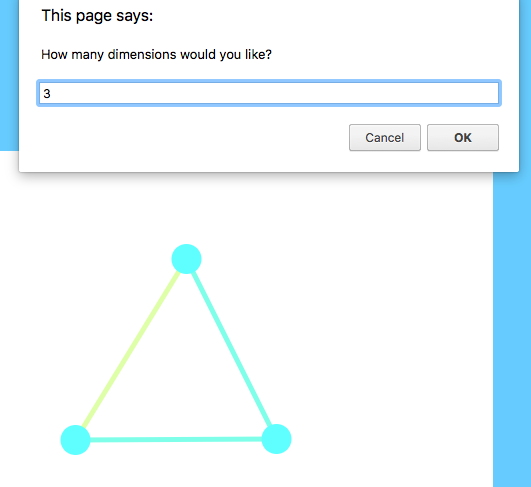
\includegraphics[width=.49\linewidth]{img/i1}
   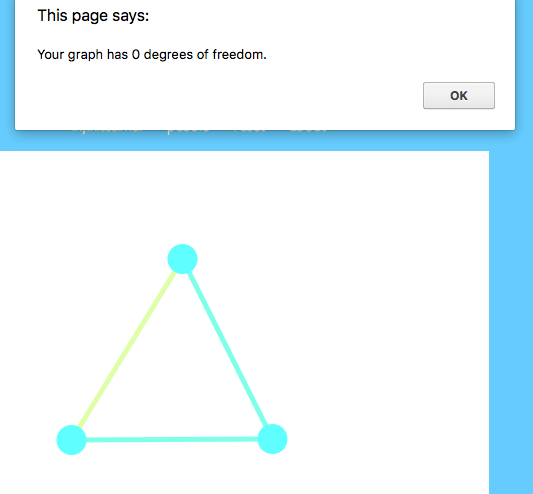
\includegraphics[width=.49\linewidth]{img/i2}
   \caption{Interface for infinitesimal rigidity.}
   \label{fig:inf}
\end{figure*}

Any graph drawn with our GUI can be tested for infinitesimal rigidity.
Though we can only draw graphs in two dimensions,
we may randomly embed them in $n$ dimensional space.
This is possible because in the infinitesimal case,
we are only concerned with the combinatorial structure of the graph.
Thus, the user is prompted to enter the desired number of dimensions
when running infinitesimal rigidity.
\Cref{fig:inf} shows this process for a triangle.

\section{Discussion}
\label{sec:discuss}

\subsection{Comparison with existing applet}


\begin{table*}[ht]
\def\arraystretch{1.5}
\caption{Comparison of Rigiditea and existing Java implementation
across different features and criteria.}
\begin{tabular}{p{0.4\linewidth} | p{0.4\linewidth}}
Rigiditea & Java implementation \\ \hline
minimalist web GUI, completely front-end, can be hosted anywhere
without a backend &
Java application, requires download to run (most systems have a JVM) \\
aesthetic design, fun to play with, keyboard shortcuts convenient &
standard software developer look, though with intuitive icons
and a thorough menu\\
draw graphs completely freehand,
with simple editing tools &
select from a set of sample graphs,
which demonstrate certain concepts \\
graphs are fixed in location and scale &
graphs can be rotated and moved around point or segment \\
visualize individual steps of pebble algorithm &
visualize individual steps of pebble algorithm\\
tests for linkage rigidity & tests for linkage rigidity\\
only provides overall rigidity & finds over-braced components \\
provides tester for infinitesimal rigidity in $n$ dimensions,
independent of the pebble algorithm
& not a design goal
\end{tabular}
\label{tab:comp}
\end{table*}


Rigiditea is not the first application to visualize linkage rigidity.
There currently exists another
implementation of the pebble algorithm as a Java application~\cite{stjohnapplet}.

Compared to Rigiditea, this implementation
has more built-in features and is a more mature application,
but as a fully front-end web application,
Rigiditea is more accessible, easy-to-use, and pleasing to look at.
Rigiditea also offers complete flexibility in graph design,
instead of using several existing shapes for demonstration purposes.
\Cref{tab:comp} provides an extensive comparison of the two implementations.
On a whole, Rigiditea is not meant to replace the existing tool,
but rather to provide a simpler tool for those casually interested
in rigidity.

Moreover, we envision Rigiditea as a means for laypersons
to learn more about rigidity in general.
Towards these aspects, we should perhaps add additional features,
but due to time constraints, we opted for just a rigidity tester.

\subsection{Future work}

While Rigiditea is currently a simple, functional web application,
there are several extensions we may explore for Rigiditea
to improve its functionality and user-friendliness.

\subsubsection{Web interface}

It would be convenient to scroll through the pebble algorithm's steps
in a timeline, similar to that of the existing Java implementation.
This feature could be easy to implement,
if we simply maintain a history of the \texttt{PebbleGraph} objects
and display one of them depending on the time step.
Afterwards, we could optimize this history by storing a log
of updates and changes to the \texttt{PebbleGraph},
rather than replicating the object $t$ times for $t$ time steps.

Furthermore, there are several GUI features that would be nice to have,
which we ran out of time to implement.
To improve our graph editing capabilities,
we should include the ability to drag nodes around with \texttt{ALT+click}.
It would also be ideal to snap nodes to a grid,
so the overall design looks neater.

Finally, it would be convenient to export graphs into the FOLD format
However, we did not prioritize this goal since
linkages can be adequately visualized as planar graphs,
which are quite conceptually general.
We also did not envision this application as a graph-sharing website,
but rather as a visual tutorial or linkage playground.
And while FOLD may also present alternative means of linkage visualization,
we are quite satisfied with ours.

\subsubsection{Algorithmic extensions}

Algorithmically, we would also like to visualize rigid components of a linkage.
It would be ideal to color the over-braced,
under-braced, and minimally rigid components so a user
can distinguish between them.
The existing Java implementation shows rigid components,
though it only applies the algorithm to a few pre-determined linkages.
The pebble algorithm can be used to determine such components,
but we did not have the time to implement that element here.

Finally, we would like to extend this web application to other pebble games
such as those presented in \cite{lee08}.
These generalize our pebble games to a whole family of $(k,\ell)$-pebble games
which test $(k,\ell)$-sparsity.
This sparsity condition rather resembles the Laman condition:
it requires that the subgraph induced by $n'$ vertices have at most $kn' - \ell$ vertices.
Indeed, the Laman condition, which our pebble algorithm tests,
is simply $(2,3)$-sparsity.


\appendix*
\section{Miscellaneous remarks}

\subsection{Challenges}

We encountered several challenges along the way.
First, Tony didn't realize his CoffeeScript didn't compile---until the ``morning''
of the presentation.
Second, Rachel didn't realize that a button would be easier to use
and infinitely easier to implement than click-and-drag.

In seriousness, both of us were new to CoffeeScript;
overzealous extrapolation from Python syntax resulted
in many unpleasant debugging experiences.

We opted to use fewer ``out-of-the-box'' \texttt{d3.js} solutions such as
the force-directed graph, so we weren't able to provide more advanced features
like bouncing our graph around and stretching edges.
However, we realized that it was more important to develop a working product,
and graphs are not typically squishy (as the force-directed graph may suggest),
so we remained with our simpler representations.

\subsection{Work distribution}

The two authors distributed the work equally.
Tony primarily worked on the pebble algorithm and infinitesimal rigidity implementations,
while Menghua designed and created the GUI.
Both contributed equally to the writing of this paper.

\subsection{Code}

A live demonstration of this application may be found at
\url{http://web.mit.edu/rmwu/www/rigid/} for the time being.
Rigiditea's source code is located in a public git repository,
\url{https://github.com/rmwu/rigiditea}.

The project was named after bubble tea since we really like bubble tea.
For the interested reader, we used many \texttt{console.log} statements
with different flavors of bubble tea to quickly track errors.
Many remain for the entertainment of confused and/or curious users.

\begin{acknowledgments}
We would like to thank Professor Erik Demaine for his instruction,
humor, and guidance. We would also like to thank the 6.849 course staff,
Martin Demaine, Dr. Jason Ku, Adam Hesterberg, and Jayson Lynch
for their continual support throughout the semester.
Finally, we would like to thank Ludwig van Beethoven for providing
music in the wee hours of the morning.
\end{acknowledgments}

\bibliography{rigiditea}{}
\bibliographystyle{plain}






\end{document}

